% Provenance (never printed): see sources/outline_sources.md (Year 1:
% geological cross-sections, apparent dip, thickness, boreholes). Every
% Varden Hills number comes from figdata/bachelor-1/varden_sections.py, which
% imports the shared model figdata/shared/region.py; numbers of the exercises
% and problem in the Book 3 scratch calculator and in that script's values.
\chapter{अनुप्रस्थ काट}\label{ch:b1:cross-sections}

एक इंजीनियरिंग कंपनी वार्डन पहाड़ियों के नीचे एक सुरंग की योजना बनाती है, जो \qty{200}{m} की स्थिर ऊँचाई पर
पश्चिम से पूर्व की ओर सीधी जाती है। एक भी मीटर खोदने से पहले भूवैज्ञानिकों को बताना होगा कि मशीन कौन-सी
चट्टानें काटेगी, वह भ्रंश को कहाँ पार करेगी, और चूना-पत्थर में, जो खुली खोखली जगहों और पानी को रख सकता है,
वह कितना समय बिताएगी। पहाड़ियों के भीतर कोई नहीं देख सकता; पर \cref{ch:b1:geological-maps} का \omterm{def:b1:geological-maps:geological-map}{भूवैज्ञानिक
मानचित्र}, कुछ बोरहोल और समतलों की ज्यामिति इतनी पर्याप्त हैं कि ज़मीन के आरपार एक ऊर्ध्वाधर टुकड़ा खींचा
जा सके --- एक अनुप्रस्थ काट --- और उससे उत्तर पढ़े जा सकें। यह अध्याय सिखाता है कि मानचित्र से काट कैसे बनती
है, तिरछी काट से नतियाँ और मोटाइयाँ कैसे बदलती हैं, बोरहोलों का \omterm{def:b1:cross-sections:log}{सहसंबंध} कैसे होता है, और काट उन चट्टानों
का इतिहास कैसे बताती है जिन्हें वह काटती है। यह सुरंग के साथ समाप्त होता है।

\begin{recall}
किसी समतल का \omterm{def:b1:geological-maps:attitude}{अभिविन्यास} उसकी \omterm{def:b1:geological-maps:attitude}{नति-दिशा} $\alpha$ और उसकी \omterm{def:b1:geological-maps:attitude}{नति} $\delta$ से दिया जाता है, और $z_0$ उन्नयन वाले
एक बिंदु से होकर, मूल-बिंदु पर, जाने वाला समतल है $z = z_0 - \tan\delta\,(x\sin\alpha + y\cos\alpha)$; किसी \omterm{def:b1:geological-maps:geological-map}{संपर्क}
के तीन बिंदु उसका \omterm{def:b1:geological-maps:attitude}{अभिविन्यास} तय करते हैं; V-नियम घाटियों में \omterm{def:b1:geological-maps:geological-map}{बहिर्भाग} के प्रारूप से \omterm{def:b1:geological-maps:attitude}{नति} पढ़ता है
(\cref{ch:b1:geological-maps})। एक समोच्च रेखा स्थलाकृतिक मानचित्र पर समान ऊँचाई के बिंदुओं को जोड़ती है
(पुस्तक 1, कक्षा 9)। नई चट्टानें पुरानी चट्टानों पर पड़ती हैं, और जो चट्टान को काटता है वह उससे नया है
(पुस्तक 1, कक्षा 7)।
\end{recall}

\section{मानचित्र से काट तक}

\begin{definition}[भूवैज्ञानिक अनुप्रस्थ काट, स्थलाकृतिक रूपरेखा, ऊर्ध्वाधर अतिरंजन]\label{def:b1:cross-sections:section}
एक \emph{भूवैज्ञानिक अनुप्रस्थ काट}\index{भूवैज्ञानिक अनुप्रस्थ काट} ज़मीन के आरपार एक ऊर्ध्वाधर समतल में
चट्टान इकाइयों और संरचनाओं का चित्र है, जो मानचित्र पर खींची गई एक रेखा के अनुदिश है। उसका ऊपरी किनारा
\emph{स्थलाकृतिक रूपरेखा}\index{स्थलाकृतिक रूपरेखा} है, यानी उस रेखा के अनुदिश ज़मीनी उन्नयन का वक्र। किसी काट का
\emph{ऊर्ध्वाधर अतिरंजन}\index{ऊर्ध्वाधर अतिरंजन} $e$ उसके ऊर्ध्वाधर पैमाने और क्षैतिज पैमाने का अनुपात है; एक
काट \emph{पैमाने के सत्य} होती है जब $e = 1$ हो।
\end{definition}

\begin{method}[मानचित्र से अनुप्रस्थ काट बनाना]\label{met:b1:cross-sections:construct}
\begin{enumerate}
  \item काट की रेखा मानचित्र पर खींचिए और कागज़ की एक पट्टी का किनारा उस पर रखिए; हर समोच्च रेखा कहाँ उसे
        पार करती है, उसका उन्नयन लिखकर अंकित कीजिए, और हर \omterm{def:b1:geological-maps:geological-map}{संपर्क} और भ्रंश कहाँ पार करता है।
  \item उतनी ही लंबाई की एक क्षैतिज आधार रेखा और उन्नयन का एक ऊर्ध्वाधर पैमाना खींचिए ($e$ चुनिए, और उसे काट पर लिखिए)।
  \item हर समोच्च-चिह्न को उसके उन्नयन पर स्थानांतरित कीजिए और बिंदुओं को सहजता से जोड़िए: यही \omterm{def:b1:cross-sections:section}{स्थलाकृतिक
        रूपरेखा} है।
  \item हर \omterm{def:b1:geological-maps:geological-map}{संपर्क} और भ्रंश को रूपरेखा पर स्थानांतरित कीजिए, उस बिंदु पर जहाँ वह रेखा को पार करता है।
  \item ऐसे हर बिंदु से \omterm{def:b1:geological-maps:geological-map}{संपर्क} को ज़मीन में उसकी \omterm{def:b1:geological-maps:attitude}{नति} के साथ खींचिए --- \emph{काट के तल में} उसकी \omterm{def:b1:geological-maps:attitude}{नति}, यानी \omterm{def:b1:cross-sections:apparent-dip}{आभासी
        नति} (\cref{sec:b1:cross-sections:apparent}) --- जिसे $e$ से बढ़ाया गया हो, यदि $e \ne 1$ हो; जहाँ बोरहोल और
        \omterm{def:b1:cross-sections:structure-contour}{संरचना समोच्च} हों, वहाँ उनका उपयोग कीजिए।
  \item संपर्कों के बीच की इकाइयाँ पूरी कीजिए, अध्यारोपण और काटों के क्रम का सम्मान करते हुए, और संकेत-सूची, पैमाने,
        रेखा की दिशा और $e$ जोड़िए।
\end{enumerate}
\end{method}

\begin{omfigure}
\begin{tikzpicture}[font=\scriptsize, x=1cm, y=1cm]
% map strip with contours crossing the section line
\draw[black!50] (0,2.7) rectangle (9,4.5);
\foreach \x/\h in {0.7/300, 1.6/350, 2.6/400, 4.1/400, 5.0/350, 5.8/300, 7.2/300, 8.2/350} {
  \draw[contour, brown!70!black] (\x-0.25,2.7) .. controls (\x+0.1,3.4) and (\x-0.1,3.8) .. (\x+0.2,4.5);
  \node[brown!60!black, above] at (\x+0.2,4.5) {\h};
}
\draw[omThm, thick] (0,3.6) node[left] {X} -- (9,3.6) node[right] {Y};
\fill[omDef] (3.4,3.6) circle (1.5pt);
\node[omDef, fill=white, inner sep=1pt, above right] at (3.4,3.62) {संपर्क};
% profile
\draw[->] (0,-0.1) -- (0,1.95) node[above] {उन्नयन (m)};
\draw (0,0) -- (9,0);
\foreach \y/\l in {0/250, 0.5/300, 1.0/350, 1.5/400} { \draw (-0.08,\y) -- (0,\y); \node[left] at (-0.08,\y) {\l}; }
\coordinate (p1) at (0.85,0.5); \coordinate (p2) at (1.75,1.0); \coordinate (p3) at (2.75,1.5);
\coordinate (p4) at (4.25,1.5); \coordinate (p5) at (5.15,1.0); \coordinate (p6) at (5.95,0.5);
\coordinate (p7) at (7.35,0.5); \coordinate (p8) at (8.35,1.0);
\foreach \i/\x in {1/0.85,2/1.75,3/2.75,4/4.25,5/5.15,6/5.95,7/7.35,8/8.35} {
  \draw[black!35, densely dotted] (\x,3.6) -- (p\i);
  \fill (p\i) circle (1.2pt);
}
\draw[thick] (0,0.2) .. controls (0.5,0.3) .. (p1) .. controls (1.3,0.8) .. (p2) .. controls (2.3,1.35) .. (p3)
  .. controls (3.5,1.85) .. (p4) .. controls (4.7,1.25) .. (p5) .. controls (5.5,0.7) .. (p6)
  .. controls (6.6,0.25) .. (p7) .. controls (7.9,0.75) .. (p8) .. controls (8.7,1.15) .. (9,1.2);
\draw[omDef, densely dotted] (3.4,3.6) -- (3.4,1.72);
\draw[omDef, thick] (3.4,1.72) -- (4.45,0.05);
\node[omDef, below right] at (4.3,-0.02) {संपर्क, उसकी आभासी नति के साथ खींचा गया};
\end{tikzpicture}

{\small काट बनाना (योजनाबद्ध): रेखा X--Y के साथ समोच्च रेखाओं के प्रतिच्छेदों को उनके उन्नयनों तक नीचे लाया
जाता है, ताकि \omterm{def:b1:cross-sections:section}{स्थलाकृतिक रूपरेखा} बने; रेखा को पार करने वाला एक \omterm{def:b1:geological-maps:geological-map}{संपर्क} रूपरेखा तक नीचे लाया जाता है और अपनी
\omterm{def:b1:cross-sections:apparent-dip}{आभासी नति} के साथ ज़मीन में खींचा जाता है।}
\end{omfigure}

काट, जो मॉडल से कंप्यूटर द्वारा बनी है, C--D रेखा के अनुदिश है, जो मानचित्र को $y = \qty{6}{km}$ पर ठीक पूर्व
की ओर पार करती है। इसमें वह \omterm{def:b1:geological-maps:fold}{अपनति} दिखती है जिसका बलुआ पत्थर और आधार का क्रोड $x \approx \qty{3.5}{km}$ पर
दिखता है, उसकी भुजाओं पर चूना-पत्थर और शेल, पूर्व की \omterm{def:b1:geological-maps:fold}{अभिनति} में खड़िया, और सामान्य भ्रंश। \qty{200}{m} पर
सुरंग रेखा, और \cref{sec:b1:cross-sections:boreholes} के बोरहोल B1, B2, B3 उस पर खींचे गए हैं।

\begin{omfigure}
\begin{tikzpicture}
\begin{axis}[x=1.4cm, y=0.0042cm, xmin=0, xmax=10, ymin=-500, ymax=650,
  axis on top, tick label style={font=\scriptsize}, label style={font=\small},
  xlabel={C से पूर्व की दूरी (km)}, ylabel={उन्नयन (m)},
  ytick={-400,-200,0,200,400,600}, clip=true]
\addplot[lith schist, draw=black, line width=0.3pt, even odd rule] table {figdata/out/bachelor-1-varden_sections-cd-unit-schist.dat};
\addplot[lith granite, draw=black, line width=0.3pt, even odd rule] table {figdata/out/bachelor-1-varden_sections-cd-unit-granite.dat};
\addplot[om lith={icsTriassic!35}{om sand}, draw=black, line width=0.3pt, even odd rule] table {figdata/out/bachelor-1-varden_sections-cd-unit-sandstone.dat};
\addplot[om lith={icsJurassic!40}{om limestone}, draw=black, line width=0.3pt, even odd rule] table {figdata/out/bachelor-1-varden_sections-cd-unit-limestone.dat};
\addplot[om lith={icsJurassic!15}{om shale}, draw=black, line width=0.3pt, even odd rule] table {figdata/out/bachelor-1-varden_sections-cd-unit-shale.dat};
\addplot[om lith={icsCretaceous!35}{om limestone}, draw=black, line width=0.3pt, even odd rule] table {figdata/out/bachelor-1-varden_sections-cd-unit-chalk.dat};
\addplot[lith alluvium, draw=black, line width=0.3pt, even odd rule] table {figdata/out/bachelor-1-varden_sections-cd-unit-alluvium.dat};
\addplot[black, line width=0.8pt] table {figdata/out/bachelor-1-varden_sections-cd-ground.dat};
\addplot[fault, line width=1.1pt] table {figdata/out/bachelor-1-varden_sections-cd-fault.dat};
\addplot[omThm, line width=1.4pt] coordinates {(1,200) (9,200)};
\node[omThm, font=\scriptsize, fill=white, inner sep=1pt, below] at (axis cs:8.3,190) {सुरंग, \qty{200}{m}};
\draw[blue!60!black, line width=0.9pt] (axis cs:1.5,-480) -- (axis cs:1.5,524);
\draw[blue!60!black, line width=0.9pt] (axis cs:3.5,-480) -- (axis cs:3.5,381);
\draw[blue!60!black, line width=0.9pt] (axis cs:5.5,-480) -- (axis cs:5.5,530);
\node[font=\scriptsize, blue!60!black, fill=white, inner sep=1pt] at (axis cs:1.5,-440) {B1};
\node[font=\scriptsize, blue!60!black, fill=white, inner sep=1pt] at (axis cs:3.5,-440) {B2};
\node[font=\scriptsize, blue!60!black, fill=white, inner sep=1pt] at (axis cs:5.5,-440) {B3};
\node[font=\small, above right] at (axis cs:0,650) {C (पश्चिम)};
\node[font=\small, above left] at (axis cs:10,650) {D (पूर्व)};
\end{axis}
\end{tikzpicture}

\smallskip
\begin{tikzpicture}
\begin{axis}[x=1.4cm, y=0.0014cm, xmin=0, xmax=10, ymin=-500, ymax=650,
  axis on top, tick label style={font=\scriptsize}, ytick={-500,0,500},
  xticklabels={}, clip=true]
\addplot[lith schist, draw=black, line width=0.2pt, even odd rule] table {figdata/out/bachelor-1-varden_sections-cd-unit-schist.dat};
\addplot[lith granite, draw=black, line width=0.2pt, even odd rule] table {figdata/out/bachelor-1-varden_sections-cd-unit-granite.dat};
\addplot[om lith={icsTriassic!35}{om sand}, draw=black, line width=0.2pt, even odd rule] table {figdata/out/bachelor-1-varden_sections-cd-unit-sandstone.dat};
\addplot[om lith={icsJurassic!40}{om limestone}, draw=black, line width=0.2pt, even odd rule] table {figdata/out/bachelor-1-varden_sections-cd-unit-limestone.dat};
\addplot[om lith={icsJurassic!15}{om shale}, draw=black, line width=0.2pt, even odd rule] table {figdata/out/bachelor-1-varden_sections-cd-unit-shale.dat};
\addplot[om lith={icsCretaceous!35}{om limestone}, draw=black, line width=0.2pt, even odd rule] table {figdata/out/bachelor-1-varden_sections-cd-unit-chalk.dat};
\addplot[lith alluvium, draw=black, line width=0.2pt, even odd rule] table {figdata/out/bachelor-1-varden_sections-cd-unit-alluvium.dat};
\addplot[black, line width=0.6pt] table {figdata/out/bachelor-1-varden_sections-cd-ground.dat};
\addplot[fault, line width=0.8pt] table {figdata/out/bachelor-1-varden_sections-cd-fault.dat};
\end{axis}
\end{tikzpicture}

{\small वार्डन पहाड़ियों की काट C--D, क्षेत्र के मॉडल से। ऊपर: \omterm{def:b1:cross-sections:section}{ऊर्ध्वाधर अतिरंजन} $e = 3$; नीचे: वही काट पैमाने
के सत्य ($e = 1$), जहाँ \ang{12} की भुजाएँ उतनी ही मंद दिखती हैं जितनी वे हैं। रंग \omterm{def:b1:geological-maps:geological-map}{भूवैज्ञानिक मानचित्र}
\cref{ch:b1:geological-maps} के अनुसार हैं; भ्रंश (मोटी रेखा) सामान्य भ्रंश है, जिसका पूर्वी खंड नीचे खिसका
है। लाल रेखा समस्या की सुरंग है; B1--B3 बोरहोल हैं।}
\end{omfigure}

\omterm{def:b1:cross-sections:section}{ऊर्ध्वाधर अतिरंजन} पतली इकाइयों और मंद उच्चावच को पढ़ने योग्य बनाता है, पर वह हर कोण को विकृत करता है: \omterm{def:b1:geological-maps:fold}{वलन} की
\ang{12} भुजाएँ ऊपरी काट में लगभग \ang{32} पर दिखती हैं। अगला अनुच्छेद ठीक बताता है कि ऐसा कैसे होता है।

\section{आभासी नति}\label{sec:b1:cross-sections:apparent}

\begin{definition}[आभासी नति]\label{def:b1:cross-sections:apparent-dip}
किसी दिए गए ऊर्ध्वाधर काट में एक समतल की \emph{आभासी नति}\index{आभासी नति} $\beta$ क्षैतिज और उस काट में समतल के
अनुरेख के बीच का कोण है। वह वास्तविक \omterm{def:b1:geological-maps:attitude}{नति} $\delta$ के बराबर होती है जब काट \omterm{def:b1:geological-maps:attitude}{नति-दिशा} के अनुदिश चलती है, और
शून्य होती है जब वह \omterm{def:b1:geological-maps:attitude}{स्ट्राइक} के अनुदिश चलती है।
\end{definition}

\begin{theorem}[आभासी नति]\label{thm:b1:cross-sections:apparent-dip}
\omterm{def:b1:geological-maps:attitude}{नति} $\delta$ और \omterm{def:b1:geological-maps:attitude}{नति-दिशा} $\alpha$ वाला एक समतल, जिसे दिगंश $\theta$ की एक ऊर्ध्वाधर काट काटती है, \omterm{def:b1:cross-sections:apparent-dip}{आभासी नति}
$\beta$ इस प्रकार दिखाता है
\[
  \tan\beta = \tan\delta\,\cos\gamma, \qquad \gamma = \alpha - \theta ,
\]
समतल दिशा $\theta$ में नीचे जाता है, जब $\cos\gamma > 0$ हो। विशेष रूप से $|\beta| \le \delta$ है, समता केवल
\omterm{def:b1:geological-maps:attitude}{नति-दिशा} के अनुदिश।
\end{theorem}

\begin{proof}
\cref{ch:b1:geological-maps} के समतल $z = z_0 - \tan\delta\,(x\sin\alpha + y\cos\alpha)$ को लीजिए। काट के
अनुदिश लंबाई $s$ का एक क्षैतिज पग, दिशा $\theta$ में, $(x, y) = s(\sin\theta, \cos\theta)$ है, अतः
$z = z_0 - s\tan\delta\,(\sin\theta\sin\alpha + \cos\theta\cos\alpha) =
z_0 - s\tan\delta\cos(\alpha - \theta)$। अनुरेख एक सीधी रेखा है जो क्षैतिज दूरी की प्रति इकाई
$\tan\delta\cos\gamma$ नीचे उतरती है: यही $\tan\beta$ है। चूँकि $|\cos\gamma| \le 1$, $|\tan\beta| \le \tan\delta$।
\end{proof}

\begin{omfigure}
\begin{tikzpicture}[font=\scriptsize, x={(1cm,0cm)}, y={(0.6cm,0.45cm)}, z={(0cm,1cm)}]
% hidden edges of the block
\draw[black!30, densely dashed] (0,0,0) -- (0,3,0) -- (4,3,0);
\draw[black!30, densely dashed] (0,3,0) -- (0,3,2);
% the oblique vertical section, from the front-left corner to the back-right one
\fill[black!10, opacity=0.7] (0,0,0) -- (4,3,0) -- (4,3,2) -- (0,0,2) -- cycle;
\draw[black!45] (0,0,0) -- (4,3,0) -- (4,3,2);
% the dipping plane, from the top-west edge down to the base
\fill[omDef!25, opacity=0.75] (0,0,2) -- (2.6,0,0) -- (2.6,3,0) -- (0,3,2) -- cycle;
\draw[omDef] (2.6,0,0) -- (2.6,3,0);
\draw[omDef, very thick] (0,0,2) -- (2.6,0,0);
\draw[omThm, very thick] (0,0,2) -- (2.6,1.95,0);
% visible edges of the block
\draw[black!70] (0,0,0) -- (4,0,0) -- (4,0,2) -- (0,0,2) -- cycle;
\draw[black!70] (0,0,2) -- (0,3,2) -- (4,3,2) -- (4,0,2);
\draw[black!70] (4,0,0) -- (4,3,0) -- (4,3,2);
% labels
\draw[omDef] (2.0,0,0) arc[start angle=180, end angle=142.4, radius=0.6cm];
\node[omDef] at (1.7,0,0.2) {$\delta$};
  \node[omDef, below, align=center] at (1.3,0,0) {सामने का फलक, नति-दिशा के अनुदिश:\\ वास्तविक नति $\delta$};
  \node[omThm, right, align=left] at (4.45,2.2,0.3) {तिर्यक काट (धूसर):\\ आभासी नति $\beta < \delta$};
  \node[above] at (0,1.5,2) {\omnameCompassN};
\draw[->] (0.15,1.5,2.05) -- (0.15,2.2,2.05);
\end{tikzpicture}

{\small \omterm{def:b1:cross-sections:apparent-dip}{आभासी नति} (योजनाबद्ध खंड)। पूर्व की ओर झुकता एक समतल (नीला) अपने सामने के फलक पर, जो \omterm{def:b1:geological-maps:attitude}{नति-दिशा}
के अनुदिश काटा गया ऊर्ध्वाधर फलक है, अपनी वास्तविक \omterm{def:b1:geological-maps:attitude}{नति} $\delta$ दिखाता है; धूसर ऊर्ध्वाधर काट पर, जो तिरछी
काटी गई है, उसका अनुरेख (लाल) अधिक मंद उतरता है, \omterm{def:b1:cross-sections:apparent-dip}{आभासी नति} $\beta$ के साथ; उत्तर-दक्षिण \omterm{def:b1:geological-maps:attitude}{स्ट्राइक} के
अनुदिश काट पर वह क्षैतिज होता।}
\end{omfigure}

\begin{proposition}[अतिरंजित काट में कोण]\label{prop:b1:cross-sections:exaggeration}
\omterm{def:b1:cross-sections:section}{ऊर्ध्वाधर अतिरंजन} $e$ के साथ बनाई गई काट में \omterm{def:b1:cross-sections:apparent-dip}{आभासी नति} $\beta$ वाली एक रेखा, कोण $\beta'$ पर खींची जाती है जिसके
लिए $\tan\beta' = e\tan\beta$।
\end{proposition}

\begin{proof}
क्षैतिज दूरी $s$ पर रेखा $s\tan\beta$ नीचे उतरती है; ऊर्ध्वाधर पैमाने को क्षैतिज पैमाने का $e$ गुना लेकर, वही
उतार $es\tan\beta$ के रूप में, उसी खींची गई लंबाई $s$ पर दिखता है।
\end{proof}

\begin{example}
वार्डन \omterm{def:b1:geological-maps:fold}{अपनति} की पूर्वी भुजा \ang{12.16} से \ang{080.7} की ओर झुकती है (\cref{ch:b1:geological-maps})। पूर्व-पश्चिम काट
C--D में, $\gamma = \ang{80.7} - \ang{90} = \ang{-9.3}$, और $\tan\beta =
\tan\ang{12.16}\cos\ang{9.3} = 0.2154\times0.9868 = 0.2126$: $\beta =
\ang{12.0}$। $e = 3$ के साथ खींची गई वह $\arctan(3\times0.2126) =
\ang{32.5}$ पर दिखती है। दिगंश \ang{071.6} की काट A--B में $\gamma = \ang{9.1}$
और $\beta = \ang{12.0}$ भी है: दोनों काटें \omterm{def:b1:geological-maps:attitude}{नति-दिशा} के निकट चलती हैं। भ्रंश, जो \ang{120} की ओर \ang{60} झुकता है,
C--D में \omterm{def:b1:cross-sections:apparent-dip}{आभासी नति} $\arctan(\tan\ang{60}\cos\ang{30}) = \arctan 1.5 = \ang{56.3}$ रखता है।
\end{example}

\section{मोटाई}

\begin{definition}[वास्तविक मोटाई, ऊर्ध्वाधर मोटाई]\label{def:b1:cross-sections:thickness}
किसी परत की \emph{वास्तविक मोटाई}\index{वास्तविक मोटाई} $t$ उसके आधार और ऊपरी सिरे के बीच की वह दूरी है जो
परत-तल के लंबवत मापी जाती है। उसकी \emph{ऊर्ध्वाधर मोटाई}\index{ऊर्ध्वाधर मोटाई} $h$ वही दूरी है जो ऊर्ध्वाधर के
अनुदिश मापी जाती है, जैसे एक ऊर्ध्वाधर बोरहोल उसे काटता है।
\end{definition}

\begin{proposition}[नत परत की मोटाई]\label{prop:b1:cross-sections:thickness}
\omterm{def:b1:geological-maps:attitude}{नति} $\delta$ वाली परत के लिए:
\begin{enumerate}
  \item $t = h\cos\delta$;
  \item क्षैतिज ज़मीन पर, यदि परत के \omterm{def:b1:geological-maps:geological-map}{बहिर्भाग} की चौड़ाई \omterm{def:b1:geological-maps:attitude}{स्ट्राइक} के लंबवत मापी गई $w$ है, तो $t = w\sin\delta$;
  \item \omterm{def:b1:geological-maps:attitude}{स्ट्राइक} के लंबवत दिशा में $\sigma$ कोण पर ढलती ज़मीन पर, जिसमें $w$ ज़मीन के अनुदिश मापा गया है,
        $t = w\sin(\delta + \sigma)$ यदि ज़मीन \omterm{def:b1:geological-maps:attitude}{नति} से विपरीत ढलती है, और $t = w\sin(\delta - \sigma)$ यदि वह \omterm{def:b1:geological-maps:attitude}{नति}
        की ही दिशा में परतों से कम तीखी ढलती है।
\end{enumerate}
\end{proposition}

\begin{proof}
\omterm{def:b1:geological-maps:attitude}{स्ट्राइक} के लंबवत ऊर्ध्वाधर समतल में परत का आधार और ऊपरी सिरा $\delta$ पर झुकी दो समांतर रेखाएँ हैं, जो $t$ दूरी
पर हैं। (1) उन्हें जोड़ने वाला एक ऊर्ध्वाधर खंड उनके सामान्य अभिलंब के साथ $\delta$ कोण बनाता है, अतः $t = h\cos\delta$।
(2)--(3) उन्हें ज़मीन के अनुदिश जोड़ने वाला लंबाई $w$ का एक खंड परत-तल के साथ, जब ज़मीन समतल हो तब $\delta$,
जब ज़मीन \omterm{def:b1:geological-maps:attitude}{नति} की विपरीत दिशा में ऊपर उठे तब $\delta + \sigma$ (दोनों झुकाव जुड़ते हैं), और जब वह उसी दिशा में
गिरे तब $\delta - \sigma$ कोण बनाता है; समांतर रेखाओं के बीच की दूरी खंड की लंबाई और उस कोण की ज्या का गुणनफल है।
\end{proof}

\begin{omfigure}
\begin{tikzpicture}[font=\scriptsize]
\pgfmathsetmacro{\d}{25}\pgfmathsetmacro{\t}{1.3}
\pgfmathsetmacro{\h}{\t/cos(\d)}\pgfmathsetmacro{\w}{\t/sin(\d)}
\pgfmathsetmacro{\X}{4.0}
\fill[icsJurassic!30] (-\w,0) -- (0,0) -- (\X,{-\X*tan(\d)}) -- (\X,{-\X*tan(\d)-\h}) -- cycle;
  \draw[thick] (0,0) -- (\X,{-\X*tan(\d)}) node[right] {परत का ऊपरी भाग};
  \draw[thick] (-\w,0) -- (\X,{-\X*tan(\d)-\h}) node[right] {आधार};
  \draw[black!70] ({-\w-0.8},0) -- (\X+0.6,0) node[right] {समतल ज़मीन};
% vertical thickness
\draw[omThm, thick, <->] (1.0,{-1.0*tan(\d)}) -- (1.0,{-1.0*tan(\d)-\h});
\node[omThm, right] at (1.0,{-1.0*tan(\d)-0.55*\h}) {$h$};
% true thickness, perpendicular to the bedding
\coordinate (A) at (2.8,{-2.8*tan(\d)});
\draw[omDef, thick, <->] (A) -- ++({-90-\d}:\t);
\node[omDef, right] at ($(A)+({-90-\d}:0.5*\t)$) {$t$};
% outcrop width on flat ground
\draw[black, thick, <->] (-\w,0.2) -- (0,0.2);
\node[above] at ({-0.5*\w},0.2) {$w$};
\draw[omThm] (1.0,0) arc[start angle=0, end angle=-\d, radius=1.0];
\node[omThm] at (1.25,-0.22) {$\delta$};
\end{tikzpicture}

{\small \omterm{def:b1:geological-maps:attitude}{स्ट्राइक} के लंबवत ऊर्ध्वाधर समतल में एक नत परत की मोटाइयाँ: \omterm{def:b1:cross-sections:thickness}{वास्तविक मोटाई} $t$, परत-तल के लंबवत; \omterm{def:b1:cross-sections:thickness}{ऊर्ध्वाधर
मोटाई} $h = t/\cos\delta$; समतल ज़मीन पर \omterm{def:b1:geological-maps:geological-map}{बहिर्भाग} की चौड़ाई $w = t/\sin\delta$ (योजनाबद्ध, $\delta = \ang{25}$ के साथ)।}
\end{omfigure}

वार्डन पहाड़ियों में ऊपर से चूना-पत्थर में प्रवेश करने वाला हर बोरहोल \qty{180}{m} कोर के आर-पार उसे काटता है: यही उसकी \omterm{def:b1:cross-sections:thickness}{ऊर्ध्वाधर मोटाई} है।
उसकी \omterm{def:b1:cross-sections:thickness}{वास्तविक मोटाई} $180\cos\ang{12.16} = \qty{176.0}{m}$ है। दो इकाइयाँ, जिनकी नतियाँ अलग हैं, एक ही \omterm{def:b1:geological-maps:geological-map}{बहिर्भाग} चौड़ाई
दिखा सकती हैं, और एक तीखी परत उस ढलान पर चौड़ा \omterm{def:b1:geological-maps:geological-map}{बहिर्भाग} दिखा सकती है जो उसके साथ चलती है: मोटाई मानचित्र से
कभी सीधे नहीं पढ़ी जाती।

\section{बोरहोल और संरचना समोच्च}\label{sec:b1:cross-sections:boreholes}

\begin{definition}[बोरहोल लॉग, सहसंबंध]\label{def:b1:cross-sections:log}
एक \emph{बोरहोल लॉग}\index{बोरहोल लॉग} गहराई के विरुद्ध उन चट्टानों का अभिलेख है जिन्हें एक बोरहोल ने पाया:
इकाइयाँ, उनके संपर्कों की गहराइयाँ, और कोई मापा गया गुण। \emph{सहसंबंध}\index{सहसंबंध (लॉगों का)} एक लॉग से
दूसरे लॉग तक उन्हीं इकाइयों और संपर्कों का मिलान है।
\end{definition}

C--D रेखा पर खोदे गए तीन बोरहोल हर इकाई के आधार की ज़मीन के नीचे ये गहराइयाँ देते हैं (डैश: \omterm{def:b1:geological-maps:geological-map}{संपर्क} ज़मीन के
ऊपर है, अपरदित):
\begin{center}
\small
\begin{tabular}{lcccccc}
\hline
बोरहोल & $x$ (km) & भू-सतह (m) & खड़िया & शेल & चूना-पत्थर & बलुआ पत्थर \\
\hline
B1 & 1.5 & 524.02 & 388.98 & 488.98 & 668.98 & 788.98 \\
B2 & 3.5 & 380.64 & --- & --- & 100.48 & 220.48 \\
B3 & 5.5 & 529.98 & 394.93 & 494.93 & 674.93 & 794.93 \\
\hline
\end{tabular}
\end{center}
B2 चूना-पत्थर में शुरू होता है, \omterm{def:b1:geological-maps:fold}{अपनति} के शिखर पर; B1 और B3 खड़िया में शुरू होते हैं, उसकी भुजाओं पर। भू-सतह के उन्नयन
से गहराइयाँ घटाने पर संपर्कों के उन्नयन मिलते हैं: चूना-पत्थर का आधार B2 में $380.64 - 100.48 = \qty{280.16}{m}$ और B3 में
$529.98 - 674.93 =
\qty{-144.95}{m}$ पर है, \qty{2}{km} पर \qty{425.11}{m} नीचे, \num{0.2126} की ढलान: ऊपर पाई गई
\ang{12.0} की \omterm{def:b1:cross-sections:apparent-dip}{आभासी नति}। B1 और B3 वही मोटाइयाँ देते हैं, \qty{100}{m} शेल, \qty{180}{m} चूना-पत्थर और \qty{120}{m} बलुआ
पत्थर: इकाइयों की दोनों भुजाओं पर एक ही \omterm{def:b1:cross-sections:thickness}{ऊर्ध्वाधर मोटाई} है।

\begin{omfigure}
\begin{tikzpicture}[font=\scriptsize, x=1cm, y=0.0045cm]
\foreach \b/\xx/\g/\c/\s/\l/\sd in {B1/0/524.02/388.98/488.98/668.98/788.98, B3/6/529.98/394.93/494.93/674.93/794.93} {
  \begin{scope}[xshift=\xx cm]
  \fill[icsCretaceous!35] (0,{\g}) rectangle (0.9,{\g-\c});
  \fill[icsJurassic!15] (0,{\g-\c}) rectangle (0.9,{\g-\s});
  \fill[icsJurassic!40] (0,{\g-\s}) rectangle (0.9,{\g-\l});
  \fill[icsTriassic!35] (0,{\g-\l}) rectangle (0.9,{\g-\sd});
  \fill[black!15] (0,{\g-\sd}) rectangle (0.9,{\g-\sd-40});
  \draw (0,{\g}) rectangle (0.9,{\g-\sd-40});
  \node[above] at (0.45,{\g}) {\b};
  \end{scope}
}
\begin{scope}[xshift=3cm]
  \fill[icsJurassic!40] (0,380.64) rectangle (0.9,280.16);
  \fill[icsTriassic!35] (0,280.16) rectangle (0.9,160.16);
  \fill[black!15] (0,160.16) rectangle (0.9,120);
  \draw (0,380.64) rectangle (0.9,120);
  \node[above] at (0.45,380.64) {B2};
\end{scope}
% correlation lines: base of limestone
\draw[omThm, dashed] (0.9,-144.96) -- (3,280.16);
\draw[omThm, dashed] (3.9,280.16) -- (6,-144.95);
\draw[omDef, dashed] (0.9,-264.96) -- (3,160.16);
\draw[omDef, dashed] (3.9,160.16) -- (6,-264.95);
% elevation axis
\draw[->] (-0.6,-320) -- (-0.6,600) node[above] {उन्नयन (m)};
\foreach \y in {-200,0,200,400} { \draw (-0.68,\y) -- (-0.6,\y); \node[left] at (-0.68,\y) {\y}; }
\foreach \c/\yy/\n in {icsCretaceous!35/400/खड़िया, icsJurassic!15/340/शेल, icsJurassic!40/280/चूना-पत्थर, icsTriassic!35/220/बलुआ पत्थर, black!15/160/आधार} {
  \fill[\c] (7.2,\yy) rectangle (7.45,\yy+36); \draw (7.2,\yy) rectangle (7.45,\yy+36);
  \node[right] at (7.45,\yy+18) {\n};
}
  \node[omThm, right] at (0.95,480) {चूना-पत्थर का आधार};
  \node[omDef, left] at (4.0,-250) {बलुआ पत्थर का आधार};
\end{tikzpicture}

{\small B1, B2 और B3 के लॉग, रेखा C--D पर, उनके वास्तविक उन्नयनों पर लटकाए गए (क्षैतिज पैमाने पर नहीं), और
उनका \omterm{def:b1:cross-sections:log}{सहसंबंध}: चूना-पत्थर (लाल) और बलुआ पत्थर (नीला) का आधार दोनों भुजाओं से B2 पर \omterm{def:b1:geological-maps:fold}{अपनति} के शिखर तक उठता है।}
\end{omfigure}

जहाँ बोरहोल बहुत हों, वहाँ एक दबे \omterm{def:b1:geological-maps:geological-map}{संपर्क} का आकार संरचना समोच्चों से मानचित्रित होता है।

\begin{definition}[संरचना समोच्च, संरचना-समोच्च मानचित्र]\label{def:b1:cross-sections:structure-contour}
किसी भूवैज्ञानिक सतह का \emph{संरचना समोच्च}\index{संरचना समोच्च} उस सतह के समान उन्नयन वाले बिंदुओं को जोड़ने वाली
रेखा है। एक \emph{संरचना-समोच्च मानचित्र}\index{संरचना-समोच्च मानचित्र} एक सतह के संरचना समोच्च नियमित अंतराल पर
खींचता है, चाहे वह सतह भूमिगत हो या अपरदन से मिट गई हो।
\end{definition}

किसी समतल के लिए \omterm{def:b1:cross-sections:structure-contour}{संरचना समोच्च} सीधे, \omterm{def:b1:geological-maps:attitude}{स्ट्राइक} के समांतर, और समान अंतर पर होते हैं: समोच्चों के बीच उन्नयन-अंतराल
$\Delta z$ क्षैतिज अंतर $\Delta z/\tan\delta$ के अनुरूप है। जहाँ कोई सतह मुड़ती है, वहाँ उसके समोच्च \omterm{def:b1:geological-maps:fold}{वलन} के चारों ओर
मुड़ जाते हैं; जहाँ कोई भ्रंश उसे काटता है, वहाँ वे रुककर विस्थापित होकर फिर शुरू होते हैं, एक अंतराल या एक अतिव्याप्ति के साथ।

\begin{method}[संरचना-समोच्च मानचित्र बनाना]\label{met:b1:cross-sections:structure-contours}
\begin{enumerate}
  \item हर बोरहोल के लिए, और हर बिंदु के लिए जहाँ सतह का \omterm{def:b1:geological-maps:geological-map}{बहिर्भाग} है, सतह का उन्नयन परिकलित कीजिए (भू-उन्नयन घटा
        गहराई; \omterm{def:b1:geological-maps:geological-map}{बहिर्भाग} पर स्वयं भू-उन्नयन)।
  \item जहाँ सतह एक समतल के निकट है, वहाँ तीन बिंदु लेकर \cref{ch:b1:geological-maps} की तीन-बिंदु विधि से उसका
        \omterm{def:b1:geological-maps:attitude}{अभिविन्यास} ज्ञात कीजिए; \omterm{def:b1:geological-maps:attitude}{स्ट्राइक} के समांतर समोच्च खींचिए, $\Delta z/\tan\delta$ दूरी पर।
  \item जहाँ नहीं है, वहाँ पड़ोसी बिंदुओं के बीच रैखिक अंतर्वेशन कीजिए (बिंदुओं के त्रिभुज), और समान उन्नयन जोड़िए।
  \item पहले भ्रंश खींचिए, और हर भ्रंश-खंड को अलग से समोच्चित कीजिए।
\end{enumerate}
\end{method}

\begin{omfigure}
\begin{tikzpicture}
\begin{axis}[axis equal image, xmin=0, xmax=10, ymin=0, ymax=8, width=0.8\linewidth, clip=false,
  tick label style={font=\scriptsize}, xlabel={पूर्व (km)}, ylabel={उत्तर (km)},
  label style={font=\small}]
\addplot[contour, black!25, opacity=0.6] table {figdata/out/shared-region-contours.dat};
\addplot[omThm!80!black, line width=0.6pt] table {figdata/out/bachelor-1-varden_sections-sc.dat};
\addplot[normal fault] table {figdata/out/shared-region-fault.dat};
\addplot[black, densely dashed, line width=0.6pt] coordinates {(0,6) (10,6)};
\node[font=\scriptsize, fill=white, inner sep=1pt, below right] at (axis cs:0.05,5.95) {C};
\node[font=\scriptsize, fill=white, inner sep=1pt, below left] at (axis cs:9.95,5.95) {D};
\addplot[only marks, mark=none, point meta=explicit symbolic, nodes near coords,
  nodes near coords style={font=\tiny, omThm!70!black, fill=white, fill opacity=0.8, text opacity=1, inner sep=0.5pt, anchor=center},
  restrict expr to domain={mod(\thisrow{z_m}+400,200)}{0:0}]
  table[x=x_km, y=y_km, meta=z_m] {figdata/out/bachelor-1-varden_sections-sc-labels.dat};
\pic at (axis cs:10.6,0.8) {northarrow};
\end{axis}
\end{tikzpicture}

{\small वार्डन पहाड़ियों में चूना-पत्थर के आधार के \omterm{def:b1:cross-sections:structure-contour}{संरचना समोच्च}, हर \qty{100}{m} पर (लाल, हर \qty{200}{m} पर अंकित),
स्थलाकृतिक समोच्चों (धूसर) के ऊपर। भुजाओं पर वे लगभग उत्तर-दक्षिण चलते हैं, \omterm{def:b1:geological-maps:attitude}{स्ट्राइक} के समांतर; नमन करते वलनों
के मोड़ों के चारों ओर वे V आकृतियाँ बनाते हैं; भ्रंश पर (निशान अवनत ओर) वे दो कटाव-रेखाओं पर रुकते हैं, जो
\omterm{def:b1:cross-sections:throw}{क्षैतिज विस्थापन} से अलग हैं, और लटकती दीवार में विस्थापित होकर फिर शुरू होते हैं। काट C--D बिंदुरेखा है।}
\end{omfigure}

\section{काट से इतिहास तक}

काट केवल यह नहीं दिखाती कि चट्टानें कहाँ हैं, बल्कि यह भी कि वे वहाँ कैसे आईं। इकाइयों के बीच के \omterm{def:b1:geological-maps:geological-map}{संपर्क} या तो
निरंतर निक्षेपण, या एक अंतराल दर्ज करते हैं।

\begin{definition}[असंगति, कोणीय असंगति, अ-संगति]\label{def:b1:cross-sections:unconformity}
एक \emph{असंगति}\index{असंगति} अपरदन या अनिक्षेपण की एक सतह है जो नई चट्टानों को पुरानी से अलग करती है, और इस प्रकार
अभिलेख में एक अंतराल दर्शाती है। एक \emph{कोणीय असंगति}\index{कोणीय असंगति} में पुरानी शय्याएँ नई शय्याओं के उनकी
अपरदित कोरों पर बिछने से पहले झुकाई या मोड़ी गई थीं, अतः शय्याओं के दोनों समूह एक कोण पर मिलते हैं। एक
\emph{अ-संगति}\index{अ-संगति} में ऊपर और नीचे की शय्याएँ समांतर होती हैं, और अंतराल केवल एक अपरदन-सतह या लुप्त जीवाश्मों
या आयु के रूप में दिखता है।
\end{definition}

\begin{definition}[भ्रंश का विस्थापन, क्षैतिज विस्थापन]\label{def:b1:cross-sections:throw}
एक भ्रंश का \emph{विस्थापन}\index{विस्थापन (भ्रंश का)} उसके आरपार एक चिह्न-सतह के विस्थापन का ऊर्ध्वाधर घटक है;
उसका \emph{क्षैतिज विस्थापन}\index{क्षैतिज विस्थापन (भ्रंश का)} क्षैतिज घटक है, जो भ्रंश की \omterm{def:b1:geological-maps:attitude}{नति-दिशा} में मापा जाता है। \omterm{def:b1:geological-maps:attitude}{नति}
$\varphi$ वाले एक नति-सरक भ्रंश के लिए,
$\text{क्षैतिज विस्थापन} = \text{विस्थापन}/\tan\varphi$।
\end{definition}

सामान्य भ्रंश, जो वार्डन पहाड़ियों का है, \ang{60} झुकता है और उसका \omterm{def:b1:cross-sections:throw}{विस्थापन} \qty{200}{m} है: उसका \omterm{def:b1:cross-sections:throw}{क्षैतिज
विस्थापन} $200/\tan\ang{60} = \qty{115.5}{m}$ है। काट C--D में, जो भ्रंश की \omterm{def:b1:geological-maps:attitude}{नति-दिशा} से तिरछी है, भ्रंश \ang{56.3} पर
दिखता है, और वही \qty{200}{m} का \omterm{def:b1:cross-sections:throw}{विस्थापन} एक \omterm{def:b1:geological-maps:geological-map}{संपर्क} के दो कटाव-सिरों को काट के अनुदिश $200/1.5 = \qty{133.3}{m}$ अलग
करता है। काट को \emph{पुनःस्थापित} करने के लिए --- यह देखने के लिए कि भ्रंश के चलने से पहले चट्टानें कैसी थीं ---
लटकती दीवार वाले खंड को भ्रंश-तल पर सरकन जितना ऊपर खिसकाया जाता है; \omterm{def:b1:geological-maps:fold}{वलन} को भी पुनःस्थापित करने के लिए, परतों
को सीधा करके, बची हुई परतें अपरदित आधार के ऊपर फिर से समतल रखी जाएँगी। एक काट को नीचे से ऊपर पढ़ने पर वार्डन
पहाड़ियों का इतिहास इस प्रकार चलता है: शिस्ट, वह ग्रेनाइट जो उसे भेदता है, अपरदन, \omterm{def:b1:cross-sections:unconformity}{कोणीय असंगति}, समतल बिछी
ऊपरी परत, \omterm{def:b1:geological-maps:fold}{वलन}, भ्रंशन, और वह अपरदन जिसने आज की पहाड़ियाँ बनाईं।

\begin{history}[सिकार पॉइंट पर हटन]
% ledger: iugs:siccar-point
स्कॉटलैंड के दक्षिण-पूर्वी तट पर सिकार पॉइंट में, प्रारंभिक सिलूरियन आयु के लगभग ऊर्ध्वाधर धूसर बलुआ पत्थर
और मडस्टोन की परतें एक अपरदन-सतह से कटी हैं और लेट डिवोनियन आयु के हल्के झुके लाल ब्रेशिया, कॉन्ग्लोमरेट और
बलुआ पत्थर से ढकी हैं। जेम्स हटन ने इस \omterm{def:b1:cross-sections:unconformity}{कोणीय असंगति} का वर्णन अपनी \emph{Theory of the Earth} में किया, जो 1788
में रॉयल सोसाइटी ऑफ़ एडिनबरा के सामने पढ़ी गई और उसकी \emph{Transactions} में छपी, फिर 1795 में एक पुस्तक में
विस्तारित हुई; सर जेम्स हॉल का एक रेखाचित्र रिकॉर्ड करता है कि हटन ने क्या देखा। निचली शय्याएँ एक समुद्र-तल पर
समतल बिछी थीं, किनारे पर खड़ी कर दी गईं, ऊपर उठाई गईं और घिसी गईं; तभी उनके आरपार ऊपरी शय्याएँ जमा हुईं, और पूरी
चीज़ फिर उठी। हर चरण के लिए उस समय से कहीं अधिक लंबी अवधि चाहिए थी जितनी किसी ने सोची थी, और इस \omterm{def:b1:geological-maps:geological-map}{बहिर्भाग}
पर हटन का पाठ अक्सर उस क्षण के रूप में उद्धृत होता है जब भूविज्ञान ने जाना कि पृथ्वी कितनी पुरानी है।
\begin{center}
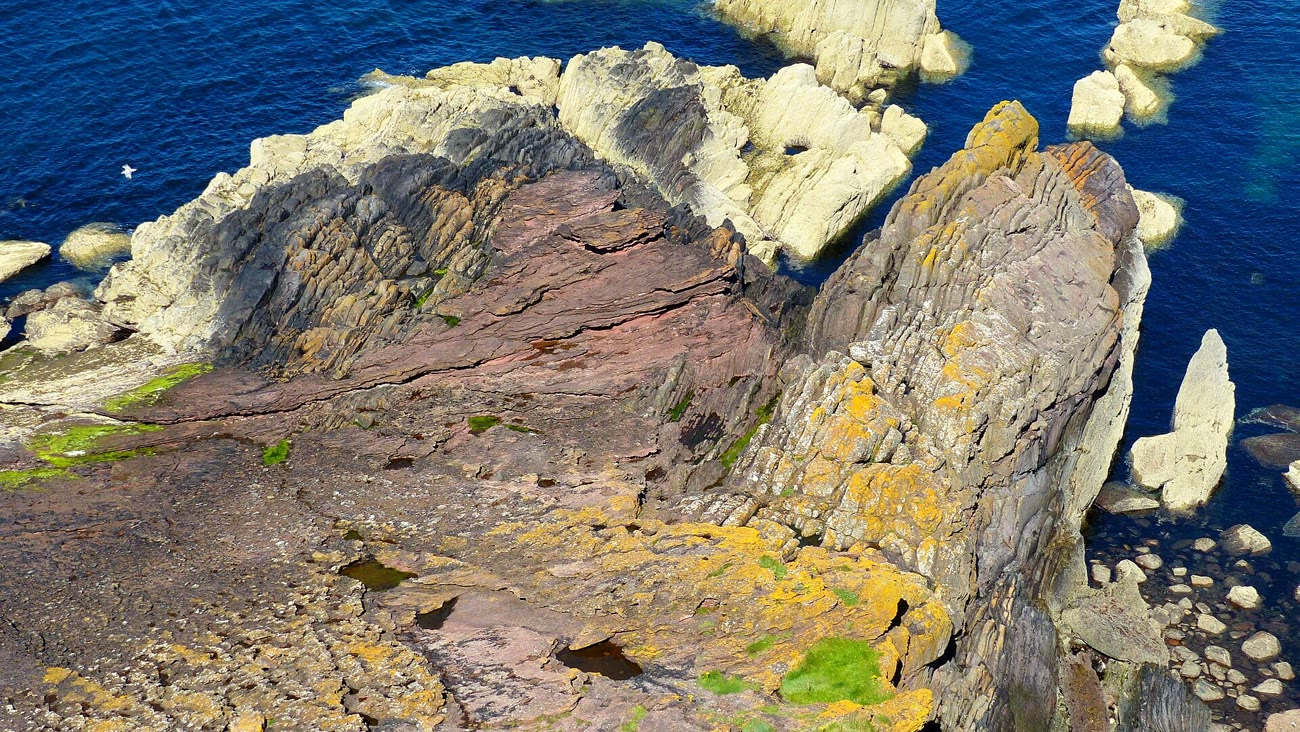
\includegraphics[width=0.7\linewidth]{images/book3/b1-siccar-point.jpg}

{\small सिकार पॉइंट पर हटन की \omterm{def:b1:cross-sections:unconformity}{असंगति}: नीचे लगभग ऊर्ध्वाधर धूसर सिलूरियन शय्याएँ, ऊपर हल्के झुकी लाल डिवोनियन
शय्याएँ। फ़ोटो: पावेल एस, CC BY-SA 4.0 (विकिमीडिया कॉमन्स)।}
% ledger: commons:siccar-point
\end{center}
\end{history}

\begin{inthefield}[सुरंग के लिए भूविज्ञान]
\begin{minipage}[t]{0.6\linewidth}\vspace{0pt}
सुरंग डिज़ाइन होने से पहले इंजीनियरिंग भूवैज्ञानिक मार्ग के साथ मानचित्र से, मार्ग के अंतरालों पर खोदे गए बोरहोलों से,
और भू-भौतिकीय सर्वेक्षणों से उसकी रेखा के अनुदिश काट बनाते हैं। वे अनुमान लगाते हैं कि सुरंग हर इकाई कहाँ
काटेगी, कौन-से भ्रंश पार करेगी, और पानी कहाँ प्रवेश कर सकता है। खुदाई के दौरान ठेकेदार के भूवैज्ञानिक हर प्रगति पर
मुख पर खुली चट्टान का लॉग रखते हैं, उसकी तुलना अनुमान से करते हैं, और काट को अद्यतन करते हैं; मशीन से आगे खोदे
गए जाँच-छेद मशीन के पहुँचने से पहले ज़मीन की परीक्षा करते हैं, विशेषकर अनुमानित भ्रंश के निकट या उस चूना-पत्थर में
जो खोखली जगहें रख सकता है। पिसी चट्टान का एक भ्रंश-क्षेत्र एक क्लासिक खतरा है, और इससे भी अधिक तब जब दोनों
ओर एक ही चट्टान हो और मुख में कुछ उसकी चेतावनी न दे।
\end{minipage}\hfill
\begin{minipage}[t]{0.37\linewidth}\vspace{0pt}
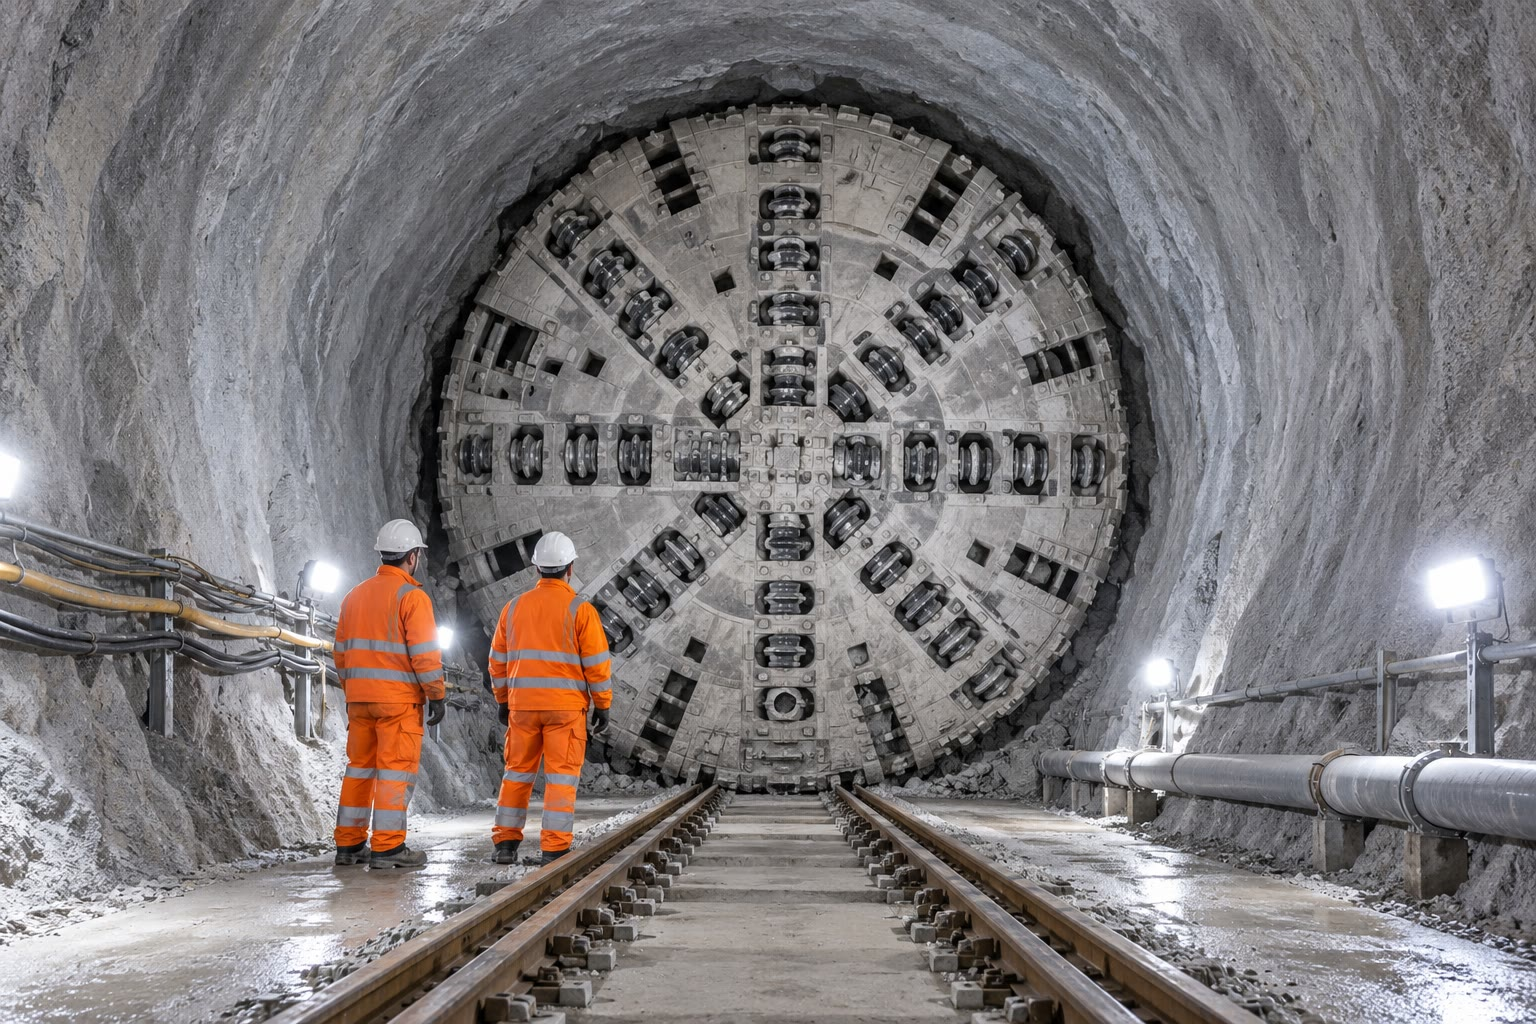
\includegraphics[width=\linewidth]{images/book3/ai/b1-tunnel-boring.jpg}
\end{minipage}
\end{inthefield}

\section{अभ्यास}

\begin{exercise}[$\star$]\label{exo:b1:cross-sections:1}
एक काट मानचित्र से 1:25\,000 पैमाने पर खींची गई है, जिसका ऊर्ध्वाधर पैमाना \qty{100}{m} के लिए \qty{1}{cm} है। उसका
\omterm{def:b1:cross-sections:section}{ऊर्ध्वाधर अतिरंजन} क्या है?
\end{exercise}

\begin{exercise}[$\star$]\label{exo:b1:cross-sections:2}
एक परत \ang{090} की ओर \ang{40} झुकती है। \ang{060} दिगंश की एक ऊर्ध्वाधर काट में उसकी \omterm{def:b1:cross-sections:apparent-dip}{आभासी नति} क्या है? \ang{000}
दिगंश की काट में?
\end{exercise}

\begin{exercise}[$\star$]\label{exo:b1:cross-sections:3}
एक ऊर्ध्वाधर बोरहोल \qty{120}{m} बलुआ पत्थर को काटता है जिसकी परतें \ang{12.16} झुकती हैं। बलुआ पत्थर की \omterm{def:b1:cross-sections:thickness}{वास्तविक मोटाई}
क्या है?
\end{exercise}

\begin{exercise}[$\star$]\label{exo:b1:cross-sections:4}
काट के तल में \ang{12} झुकता एक \omterm{def:b1:geological-maps:geological-map}{संपर्क} 2, 3 और 5 के ऊर्ध्वाधर अतिरंजनों के साथ खींचा गया है। वह किन कोणों पर दिखता है?
\end{exercise}

\begin{exercise}[$\star\star$]\label{exo:b1:cross-sections:5}
एक परत \ang{25} झुकती है। उसका \omterm{def:b1:geological-maps:geological-map}{बहिर्भाग} \qty{300}{m} चौड़ा है, जो \omterm{def:b1:geological-maps:attitude}{स्ट्राइक} के लंबवत मापा गया है। उसकी \omterm{def:b1:cross-sections:thickness}{वास्तविक मोटाई}
परिकलित कीजिए (क) समतल ज़मीन पर; (ख) ऐसी ज़मीन पर जो \omterm{def:b1:geological-maps:attitude}{नति} की विपरीत दिशा में \ang{10} ढलती है, चौड़ाई ज़मीन के
अनुदिश मापी गई हो; (ग) ऐसी ज़मीन पर जो \omterm{def:b1:geological-maps:attitude}{नति} की ही दिशा में \ang{10} ढलती है।
\end{exercise}

\begin{exercise}[$\star\star$]\label{exo:b1:cross-sections:6}
एक परत उत्तर-दक्षिण काट में उत्तर की ओर \ang{20} की \omterm{def:b1:cross-sections:apparent-dip}{आभासी नति}, और पूर्व-पश्चिम काट में पूर्व की ओर \ang{30} की
\omterm{def:b1:cross-sections:apparent-dip}{आभासी नति} दिखाती है। उसकी \omterm{def:b1:geological-maps:attitude}{नति-दिशा} और उसकी वास्तविक \omterm{def:b1:geological-maps:attitude}{नति} ज्ञात कीजिए।
\end{exercise}

\begin{exercise}[$\star\star$]\label{exo:b1:cross-sections:7}
पूर्वी भुजा पर चूना-पत्थर का आधार \ang{12.16} झुकता है। \qty{100}{m} पर खींचे गए उसके संरचना समोच्चों का क्षैतिज
अंतराल क्या है? \omterm{def:b1:cross-sections:structure-contour}{संरचना-समोच्च मानचित्र} पर उसकी जाँच कीजिए।
\end{exercise}

\begin{exercise}[$\star\star$]\label{exo:b1:cross-sections:8}
बोरहोल सारणी से B1 और B3 में शेल के आधार का उन्नयन परिकलित कीजिए। B2 के ऊपर शेल अपरदित हो गया है: चूना-पत्थर की
\omterm{def:b1:cross-sections:thickness}{ऊर्ध्वाधर मोटाई} से ज्ञात कीजिए कि वहाँ उसके आधार का उन्नयन क्या होता, और काट C--D में B1 और B2 के बीच उस \omterm{def:b1:geological-maps:geological-map}{संपर्क} की
\omterm{def:b1:cross-sections:apparent-dip}{आभासी नति} क्या है। B1 और B3 की तुलना \omterm{def:b1:geological-maps:fold}{वलन} के बारे में क्या बताती है?
\end{exercise}

\begin{exercise}[$\star\star$]\label{exo:b1:cross-sections:9}
\ang{180} की ओर \ang{50} झुकने वाला एक सामान्य भ्रंश \qty{150}{m} का \omterm{def:b1:cross-sections:throw}{विस्थापन} रखता है। उसका \omterm{def:b1:cross-sections:throw}{क्षैतिज विस्थापन}
परिकलित कीजिए। \ang{150} दिगंश की ऊर्ध्वाधर काट में भ्रंश की \omterm{def:b1:cross-sections:apparent-dip}{आभासी नति} और काट के अनुदिश एक क्षैतिज परत के दो
कटाव-सिरों का अलगाव क्या है?
\end{exercise}

\begin{exercise}[$\star\star\star$]\label{exo:b1:cross-sections:10}
\ang{40} झुकती एक परत के लिए, किन काट-दिशाओं में \omterm{def:b1:cross-sections:apparent-dip}{आभासी नति} वास्तविक \omterm{def:b1:geological-maps:attitude}{नति} की आधी, यानी \ang{20}, है? दिखाइए कि
\omterm{def:b1:cross-sections:apparent-dip}{आभासी नति} \omterm{def:b1:geological-maps:attitude}{नति-दिशा} के निकट कम और \omterm{def:b1:geological-maps:attitude}{स्ट्राइक} के निकट तेज़ी से बदलती है।
\end{exercise}

\begin{exercise}[$\star\star\star$]\label{exo:b1:cross-sections:11}
एक बोरहोल पूर्वी भुजा के चूना-पत्थर को काटता है (\omterm{def:b1:cross-sections:thickness}{वास्तविक मोटाई} \qty{176.0}{m}, \ang{080.7} की ओर \ang{12.16} \omterm{def:b1:geological-maps:attitude}{नति})।
वह कितनी लंबाई का कोर लौटाता है (क) यदि ऊर्ध्वाधर हो; (ख) यदि क्षैतिज से नीचे \ang{60} पर \ang{260.7} की ओर झुका हो;
(ग) \ang{60} पर \ang{080.7} की ओर झुका हो? (संकेत: लंबाई $t/\cos\psi$ है, जहाँ $\psi$ बोरहोल और परत-तल के अभिलंब
के बीच का कोण है।)
\end{exercise}
\begin{exercise}[$\star\star\star$]\label{exo:b1:cross-sections:12}
एक \omterm{def:b1:cross-sections:unconformity}{कोणीय असंगति} पर, नीचे की शय्याएँ \ang{090} की ओर \ang{70} झुकती हैं और ऊपर की शय्याएँ \ang{270} की ओर \ang{20},
समान \omterm{def:b1:geological-maps:attitude}{स्ट्राइक} के साथ। पूरे \omterm{def:b1:geological-maps:geological-map}{बहिर्भाग} को \omterm{def:b1:geological-maps:attitude}{स्ट्राइक} के परितः घुमाकर ऊपरी शय्याओं को क्षैतिज कीजिए: जब ऊपरी शय्याएँ जमा
हुईं, तब निचली शय्याओं की \omterm{def:b1:geological-maps:attitude}{नति} क्या थी? \omterm{def:b1:geological-maps:geological-map}{बहिर्भाग} का इतिहास क्रम से लिखिए।
\end{exercise}

\section{समस्या: वार्डन पहाड़ियों के नीचे एक सुरंग}
\begin{problem}[{सप्ताहांत समस्या --- कौन-सी चट्टानें सुरंग काटेगी, वह भ्रंश से कहाँ मिलेगी, और वह कितना चूना-पत्थर खोदेगी}]
\label{pb:b1:cross-sections:1}
% numbers from figdata/bachelor-1/varden_sections.py (model region.py) and the scratch calculator
सुरंग रेखा C--D ($y = \qty{6}{km}$) के साथ ठीक पूर्व की ओर चलती है, \qty{200}{m} की स्थिर ऊँचाई पर, $x = \qty{1}{km}$ से
$x =
\qty{9}{km}$ तक। C--D के साथ भू-उन्नयन, $x = 0$ से हर किलोमीटर पर, है:
\begin{center}
\small
\begin{tabular}{lccccccccccc}
\hline
$x$ (km) & 0 & 1 & 2 & 3 & 4 & 5 & 6 & 7 & 8 & 9 & 10 \\
$z$ (m) & 509 & 556 & 467 & 370 & 435 & 534 & 501 & 455 & 406 & 339 & 405 \\
\hline
\end{tabular}
\end{center}
अध्याय की बोरहोल सारणी, $e = 3$ के साथ खींची गई काट C--D, पूर्वी भुजा का \omterm{def:b1:geological-maps:attitude}{अभिविन्यास} (\ang{12.16} \omterm{def:b1:geological-maps:attitude}{नति}, \ang{080.7} की
ओर; पश्चिमी भुजा उसका दर्पण-प्रतिबिंब है, \ang{279.3} की ओर झुकती हुई), और सामान्य भ्रंश का उपयोग कीजिए, जो \ang{120}
की ओर \ang{60} झुकता है, \qty{200}{m} का \omterm{def:b1:cross-sections:throw}{विस्थापन} रखता है, और बिंदु $x = \qty{4.30}{km}$, $y = \qty{1.00}{km}$, $z = \qty{250}{m}$
से होकर जाता है।

\medskip
\noindent\textbf{भाग I --- स्थलाकृति और इकाइयाँ।}
\begin{enumerate}
  \item $x = 1$ और $x = 9$ के बीच के किलोमीटर बिंदुओं पर सुरंग के ऊपर चट्टान की सबसे बड़ी और सबसे छोटी मोटाइयाँ क्या हैं?
  \item मुद्रित काट पर \qty{1}{km} क्षैतिज दूरी \qty{1.4}{cm} और \qty{1}{km} उन्नयन \qty{4.2}{cm} मापता है। जाँचिए कि $e = 3$ है।
  \item B2 के लॉग से, \omterm{def:b1:geological-maps:fold}{अपनति} के शिखर पर बलुआ पत्थर के आधार का उन्नयन ज्ञात कीजिए।
  \item $x = \qty{3.5}{km}$ पर सुरंग किस इकाई में है?
  \item B1 और B3 में चूना-पत्थर के आधार का उन्नयन परिकलित कीजिए।
  \item काट से, $x = 1$ से $x = \qty{9}{km}$ तक सुरंग जिन इकाइयों को पार करती है, उन्हें क्रम में सूचीबद्ध कीजिए।
\end{enumerate}

\medskip
\noindent\textbf{भाग II --- काट में नतियाँ।}
\begin{enumerate}[resume]
  \item उसके \omterm{def:b1:geological-maps:attitude}{अभिविन्यास} से C--D में पूर्वी भुजा की \omterm{def:b1:cross-sections:apparent-dip}{आभासी नति} परिकलित कीजिए।
  \item B2 और B3 में चूना-पत्थर के आधार के उन्नयनों से उसकी जाँच कीजिए।
  \item $e = 3$ के साथ काट में पूर्वी भुजा किस कोण पर खींची गई है?
  \item C--D में भ्रंश की \omterm{def:b1:cross-sections:apparent-dip}{आभासी नति} परिकलित कीजिए।
  \item C--D में भुजाओं की \omterm{def:b1:cross-sections:apparent-dip}{आभासी नति} उनकी वास्तविक \omterm{def:b1:geological-maps:attitude}{नति} के इतनी निकट क्यों है, और भ्रंश की कम निकट क्यों?
\end{enumerate}

\medskip
\noindent\textbf{भाग III --- भ्रंश।}
\begin{enumerate}[resume]
  \item दिखाइए कि समतल $y = \qty{6}{km}$ पर भ्रंश
        \[ x = 4300 + \frac{2500 - (z - 250)\tan\ang{30}}{\sin\ang{120}}
           \quad\text{(मीटर में)}. \]
        पर स्थित है।
  \item सुरंग भ्रंश से कहाँ मिलती है?
  \item भ्रंश का \omterm{def:b1:cross-sections:throw}{क्षैतिज विस्थापन}, और C--D के किसी \omterm{def:b1:geological-maps:geological-map}{संपर्क} के कटाव-सिरों का अलगाव परिकलित कीजिए।
  \item कौन-सा खंड नीचे खिसका है, और भ्रंश के हर ओर सुरंग के स्तर पर कौन-सी इकाई है?
  \item भ्रंश एक ऐसा खतरा क्यों है जिसे सुरंग-दल मुख की चट्टान से आते नहीं देख सकता था? इंजीनियर इससे कैसे बचते हैं?
\end{enumerate}

\medskip
\noindent\textbf{भाग IV --- चूना-पत्थर।}
\begin{enumerate}[resume]
  \item B1 में चूना-पत्थर की \omterm{def:b1:cross-sections:thickness}{ऊर्ध्वाधर मोटाई} क्या है?
  \item उसकी \omterm{def:b1:cross-sections:thickness}{वास्तविक मोटाई} क्या है?
  \item दिखाइए कि C--D पर भ्रंश के पश्चिम में बलुआ पत्थर का आधार
        \[ z_b = 160.16 - |x - 3500|\tan\ang{12.0} \quad\text{(मीटर में)}. \]
        पर है।
  \item सुरंग चूना-पत्थर में तब है जब उसका आधार \qty{200}{m} से नीचे और ऊपरी सिरा ऊपर हो। दिखाइए कि यह
        $377.1 < |x - 3500|
        < 1224.0$ के लिए होता है।
  \item वे चार बिंदु दीजिए जहाँ सुरंग चूना-पत्थर में प्रवेश करती है और उससे निकलती है।
  \item दिखाइए कि हर भुजा पर खोदी गई लंबाई $h/\tan\beta$ है, जहाँ $h$ \omterm{def:b1:cross-sections:thickness}{ऊर्ध्वाधर मोटाई} और $\beta$ \omterm{def:b1:cross-sections:apparent-dip}{आभासी नति} है, और उसे परिकलित कीजिए।
  \item सुरंग कुल कितनी लंबाई का चूना-पत्थर खोदती है?
\end{enumerate}
\end{problem}
